% \subsection{Python, Sympy, Numpy, Scipy y Matplotlib}

% El lenguaje de programación Python está por defecto desprovisto de capacidades de cálculo científico e ingenieril.  Esta es una decisión de diseño para hacer que tales funcionalidades deban ser agregadas por bibliotecas especializadas. El efecto de esta decisión es que el desarrollo de las mismas corre por cuenta de usuarios que las aplican en diversos ámbitos del desarrollo científico-tecnológico antes que por profesionales de las informática.

% Las funciones del cálculo simbólico las provee la biblioteca Sympy. Se aprovecha en particular su módulo Mechanics que facilita la generación de ecuaciones para la dinámica de sistemas de cuerpos rígidos con múltiples grados de libertad y en variados sistemas de referencia \cite{sympy}.

% Los sistemas de ecuaciones diferenciales se resuelven por métodos numéricos apoyados en las funciones para la manipulación de elementos algebraicos de la biblioteca Numpy \cite{numpy} y de los algoritmos de optimización e integración numérica de Scipy \cite{SciPy}.

% El análisis en ingeniería de resultados numéricos son usualmente interpretados con representaciones gráficas. Esta capacidad la proveen las funciones de la biblioteca Matplotilb \cite{matplotlib}.


\subsection{Python, Sympy, Numpy, Scipy and Matplotlib}
The Python programming language is by default devoid of scientific and engineering calculation capabilities.
This is a design decision to make such functionalities be added by specialized libraries.
The effect of this decision is that the development of these libraries is carried out by users who apply them in various fields of scientific-technological development rather than by computer professionals.

The functions of symbolic calculation are provided by the Sympy library. Its Mechanics module is particularly useful for generating equations for the dynamics of rigid body systems with multiple degrees of freedom and in various reference systems \cite{sympy}.

Differential equation systems are solved by numerical methods supported by functions for the manipulation of algebraic elements of the Numpy library \cite{numpy} and the numerical optimization and integration algorithms of Scipy \cite{SciPy}.

Engineering analysis of numerical results is usually interpreted with graphical representations. This capability is provided by the functions of the Matplotilb library \cite{matplotlib}.




% \subsection{Cuadernos de Jupyter}

% El entorno usado en el curso para ejecutar código es la aplicación basada en la web del Proyecto Jupyter llamada JupyterLab cuyo  formato de documento es el cuaderno (notebook) Jupyter \cite{Kluyver2016jupyter}. Este alterna secciones independientes denominadas celdas. Las de entrada son de código (en variados lenguajes, Python es solo uno de los posibles) o de  anotaciones, como muestra la figura \ref{fig:jupyter}. Esta última variante de celdas se escriben en el lenguaje de  marcado Markdown \cite{markdown} que permite incrustar: texto y/o expresiones matemáticas en formato \LaTeX intercaladas, y contenido multimedia: enlaces web, imágenes, reproductores de video o sonido.

% \begin{figure}[!ht]
% \centering
% 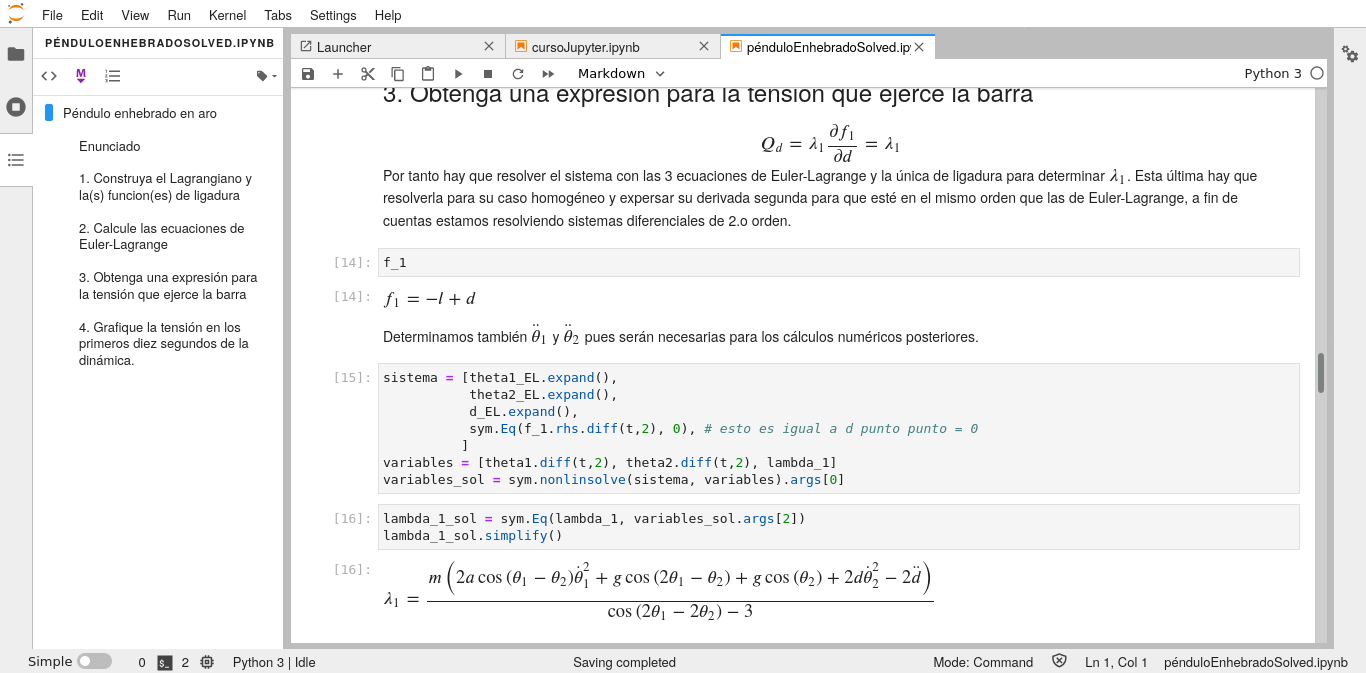
\includegraphics[width=3.5in]{figuras/screenshot_JupyterLab.png}
% \caption{Un cuaderno de Jupyter es un conjunto de celdas. Estas son en formato Markdown o de código ejecutable. Las primeras pueden contener texto,  expresiones  matemáticas o contenido multimedia. Las segundas líneas de código en variados lenguajes de programación. Intercalando títulos en las celdas Markdown se genera el índice (a la izquierda) que facilita la ubicación dentro del documento.}
% \label{fig:jupyter}
% \end{figure}

% La utilización de sintaxis \LaTeX para la simbología matemática provee una notación clara estandarizada bajo los lineamientos de la American Mathematical Society \cite{ams}.
% El resultado de la ejecución de una celda de código muestra al usuario el resultado que el mismo instruye a la computadora imprimir. En el curso estas últimas incluyen tanto los comandos para realizar cálculos así como la resolución de un sistema de ecuaciones no lineales que se imprime en la última celda del cuaderno mostrado en la figura 2.  



\subsection{Jupyter Notebooks}
The environment used in the course to run code is the web-based application of the Jupyter Project called JupyterLab, whose document format is the Jupyter notebook \cite{Kluyver2016jupyter}.
This alternates independent sections called cells.
Input cells are code (in various languages, Python is just one of the possibilities) or annotations, as shown in Figure \ref{fig:jupyter}.
This latter variant of cells is written in the Markdown markup language \cite{markdown} that allows you to embed: text and/or mathematical expressions in \LaTeX format interspersed, and multimedia content: web links, images, video and/or sound players.


\begin{figure}[!ht]
	\centering
	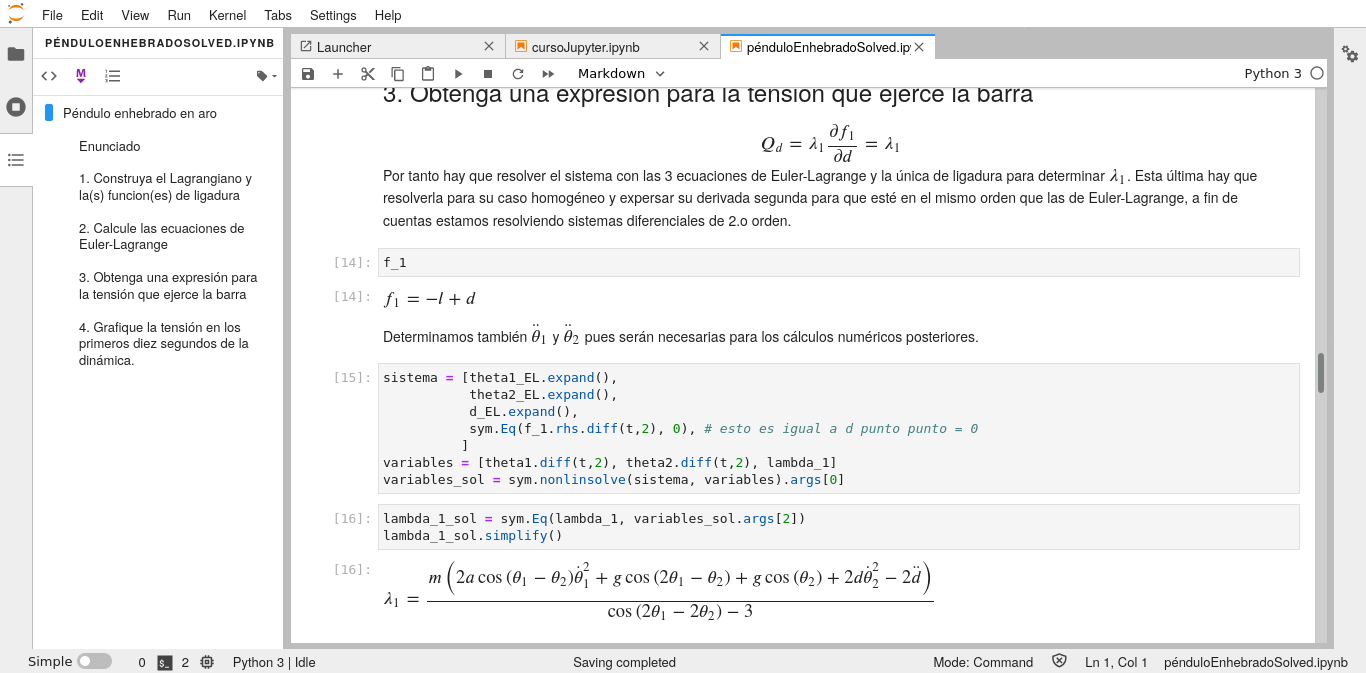
\includegraphics[width=3.5in]{figuras/screenshot_JupyterLab.png}
	\caption{
		A Jupyter notebook is a set of cells.
		These are in Markdown or executable code format.
		The former can contain text, mathematical expressions or multimedia content.
		The latter are lines of code in various programming languages.
		Interspersing titles in Markdown cells generates the index (on the left) that facilitates location within the document.
	}
	\label{fig:jupyter}
\end{figure}



% \subsection{Ejecución de Jupyter en línea}
% No se impone a los estudiantes el instalar ningún software para cursar la materia en su dispositivo informático. Solo requieren utilizar un navegador web estándar para utilizar alguno de los servicios que ejecutan cuadernos de Jupyter en línea. Este puede tratarse de una instalación de JupyterHub del Proyecto Jupyter en servidores propios de la universidad o en nubes comerciales, o en su defecto de alguno de los servicios que ofrecen alternativas incluso gratuitas como, entre otras, CoCalc, IBM Watson o Google Colaboratory. De estas se ha utilizado esta última en las últimas ediciones del curso tras cerrar Microsoft su servicio gratuito Azure Notebooks.

% El servicio Google Colaboratory, coloquialmente sólo Colab,  presenta como conveniencia el poder ejecutar cuadernos alojados en un repositorio Git gerenciado por el servicio en línea GitHub. Basta una modificación en el URL de un cuaderno para que este apunte a un navegador web a ejecutarle en Colab \cite{colab}. El trabajo con cuadernos Jupyter en este servicio puede realizarse en forma concurrente por parte de varios alumnos y/o docentes. También pueden incluirse comentarios cuya actualización es reportada por correo electrónico lo que es útil para la corrección de los ejercicios pues pueden indicarse la ubicación de errores en el código como muestra la figura \ref{fig:colab}.

%\begin{figure}[!ht]
%	\centering
%	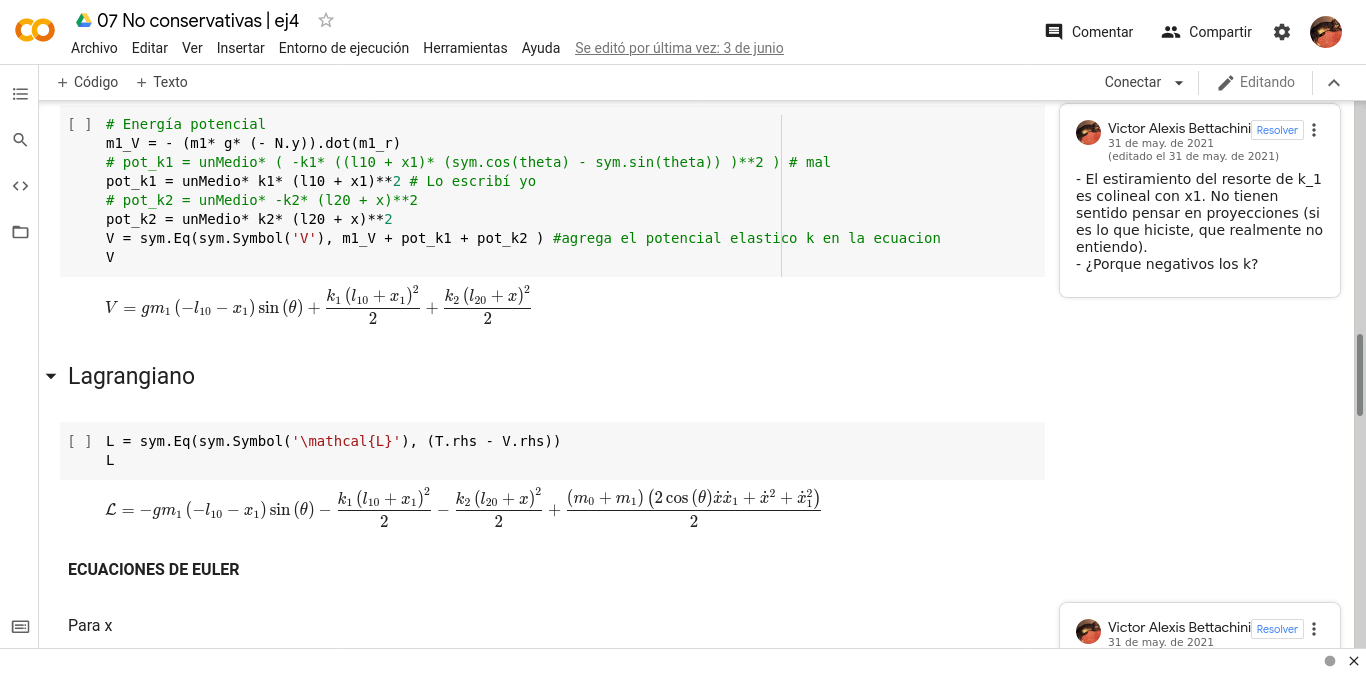
\includegraphics[width=3.5in]{figuras/comentariosColab.png}
%	\caption{
%		El sitio web Google Colaboratoy permite editar y ejecutar cuadernos Jupyter en forma concurrente entre alumnos y docentes además de incluir comentarios.
%		Esta última característica es útil para las correcciones.
%	}
%	\label{fig:colab}
%\end{figure}


\subsection{Running Jupyter Online}
Students are not required to install any software on their computer to take the course.
They only need to use a standard web browser to use one of the services that run Jupyter notebooks online.
This can be an installation of JupyterHub from the Jupyter Project on university-owned servers or commercial clouds, or alternatively one of the services that offer even free alternatives such as CoCalc, IBM Watson or Google Colaboratory.
Of these, the latter has been used in the latest editions of the course after Microsoft closed its free Azure Notebooks service.

The Google Colaboratory service, colloquially only Colab, presents as a convenience the ability to run notebooks hosted in a Git repository managed by the online service GitHub.
A modification in the URL is enough to point a notebook to a web browser to run it in Colab \cite{colab}.
Working with Jupyter notebooks in this service can be done concurrently by several students and/or teachers.
Comments can also be included, whose update is reported by email, which is useful for correcting exercises since the location of errors in the code can be indicated, as shown in Figure \ref{fig:colab}.

\begin{figure}[!ht]
	\centering
	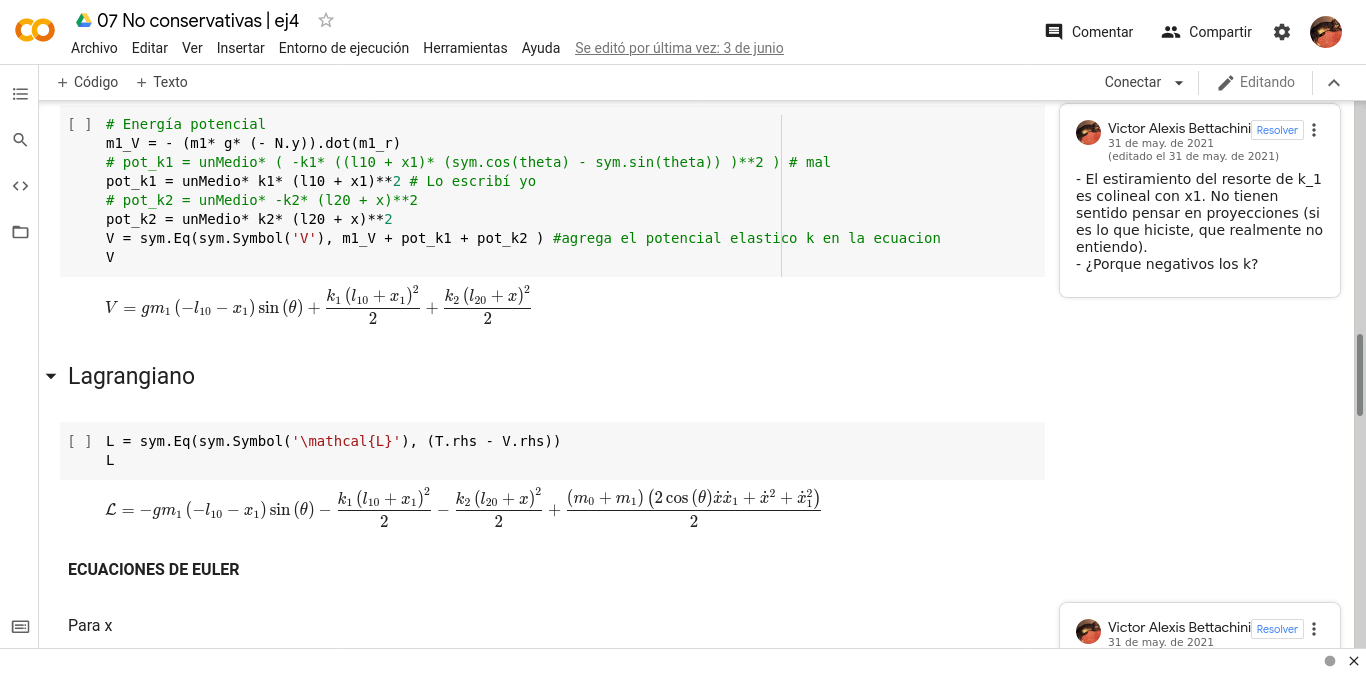
\includegraphics[width=3.5in]{figuras/comentariosColab.png}
	\caption{
		The Google Colaboratoy website allows Jupyter notebooks to be edited and run concurrently between students and teachers, as well as including comments.
		The latter feature is useful for corrections.
	}
	\label{fig:colab}
\end{figure}


% \subsection{Repositorio Git}

% El mencionado repositorio en GitHub está organizado en sendas carpetas por clase del curso, como muestra la figura \ref{fig:github}. Cada una de estas aloja el correspondiente material teórico y ejercicios en el formato de cuadernos Jupyter además de  guías de ejercicios y algún apunte ocasional en el formato de documento portátil conocido por su sigla en inglés PDF. Este ordenamiento facilita tanto al docente como a los alumnos una vista de conjunto del material de cada temática así como el verificar las eventuales actualizaciones del mismo. De esta forma el material del curso es de acceso público haciéndolo disponible para ser utilizado a interesados \cite{repositorio-victor} mientras cumplan con citar su origen y no darle uso comercial como indica su licencia Creative Commons CC-BY-NC-SA bajo el que está publicado \cite{creative}.

% \begin{figure}[!ht]
% \centering
% 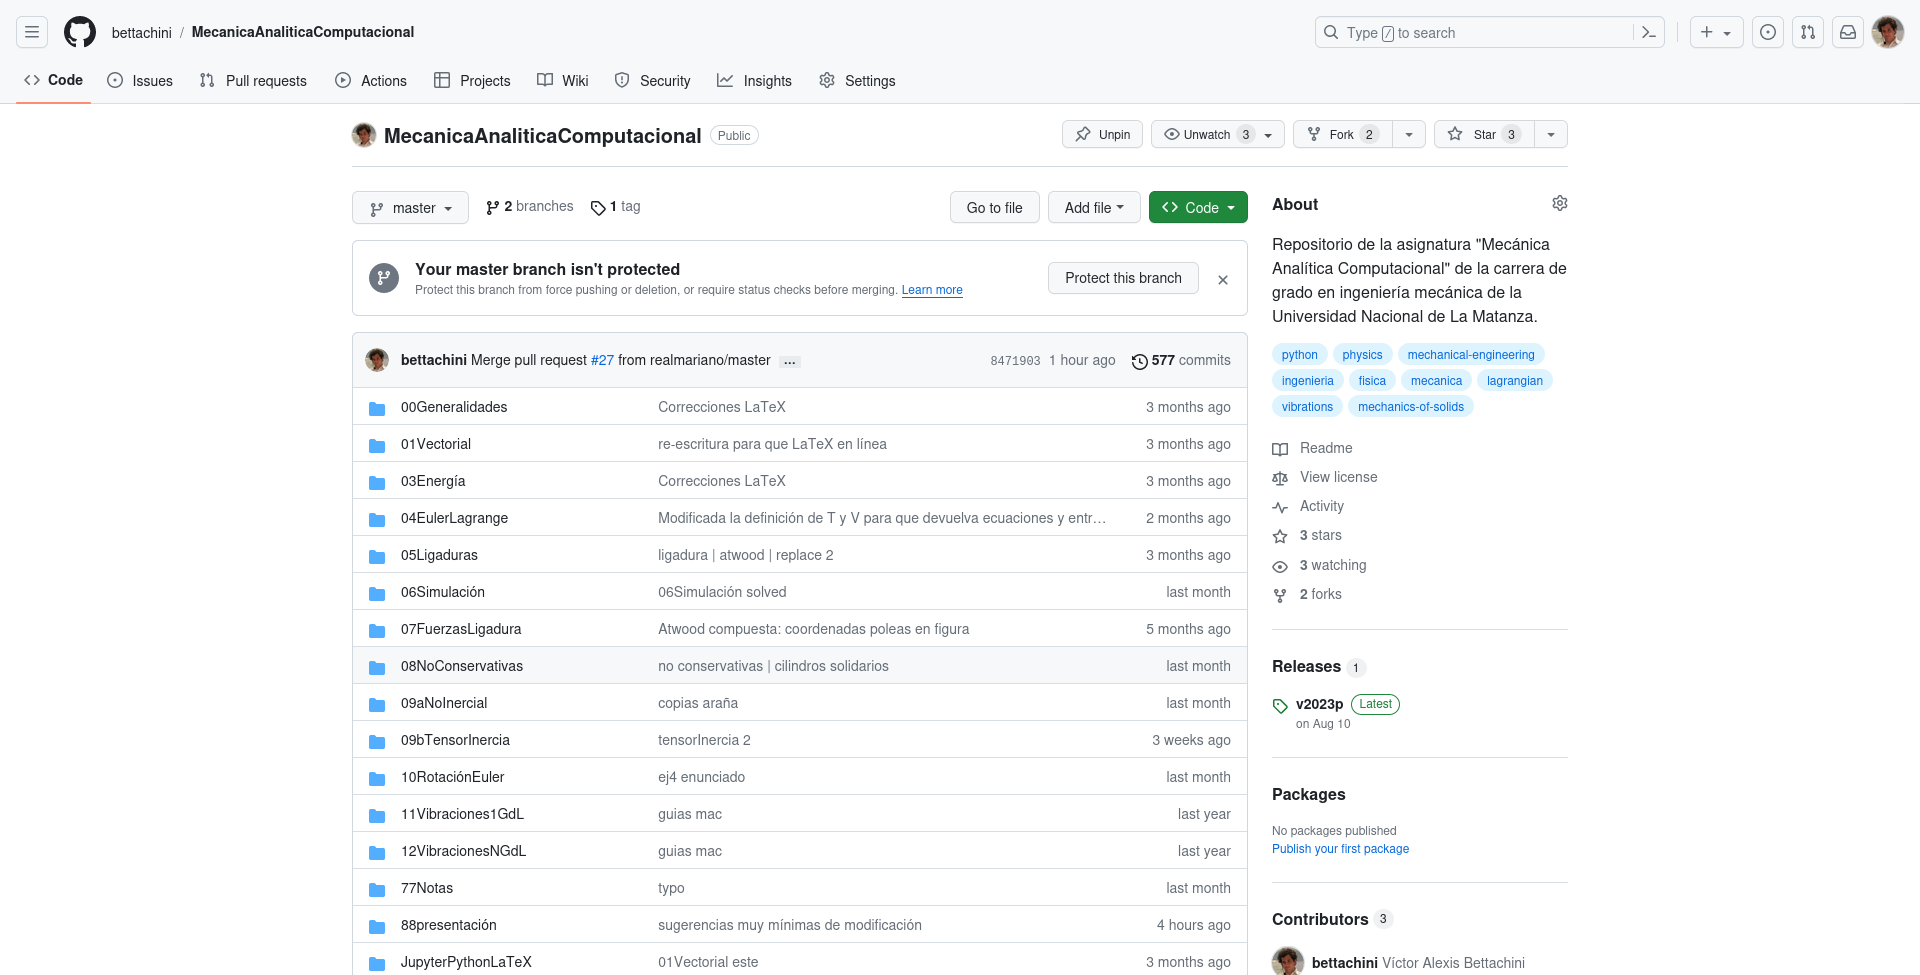
\includegraphics[width=3.5in]{figuras/repositorioGithub.png}
% \caption{Los alumnos encuentran el material ordenado en sendos directorios por clase.}
% \label{fig:github}
% \end{figure}


\subsection{Git Repository}
The aforementioned repository on GitHub is organized into separate folders for each class of the course, as shown in Figure \ref{fig:github}.
Each of these hosts the corresponding theoretical material and exercises in the format of Jupyter notebooks, as well as exercise guides and occasional notes in the portable document format known by its acronym in English PDF.
This arrangement facilitates both the teacher and the students an overview of the material of each topic as well as verifying any updates to it.
In this way, the course material is publicly accessible, making it available for use by interested parties \cite{repositorio-victor} as long as they cite its origin and do not use it commercially as indicated by its Creative Commons CC-BY-NC-SA license under which it is published \cite{creative}.

\begin{figure}[!ht]
\centering
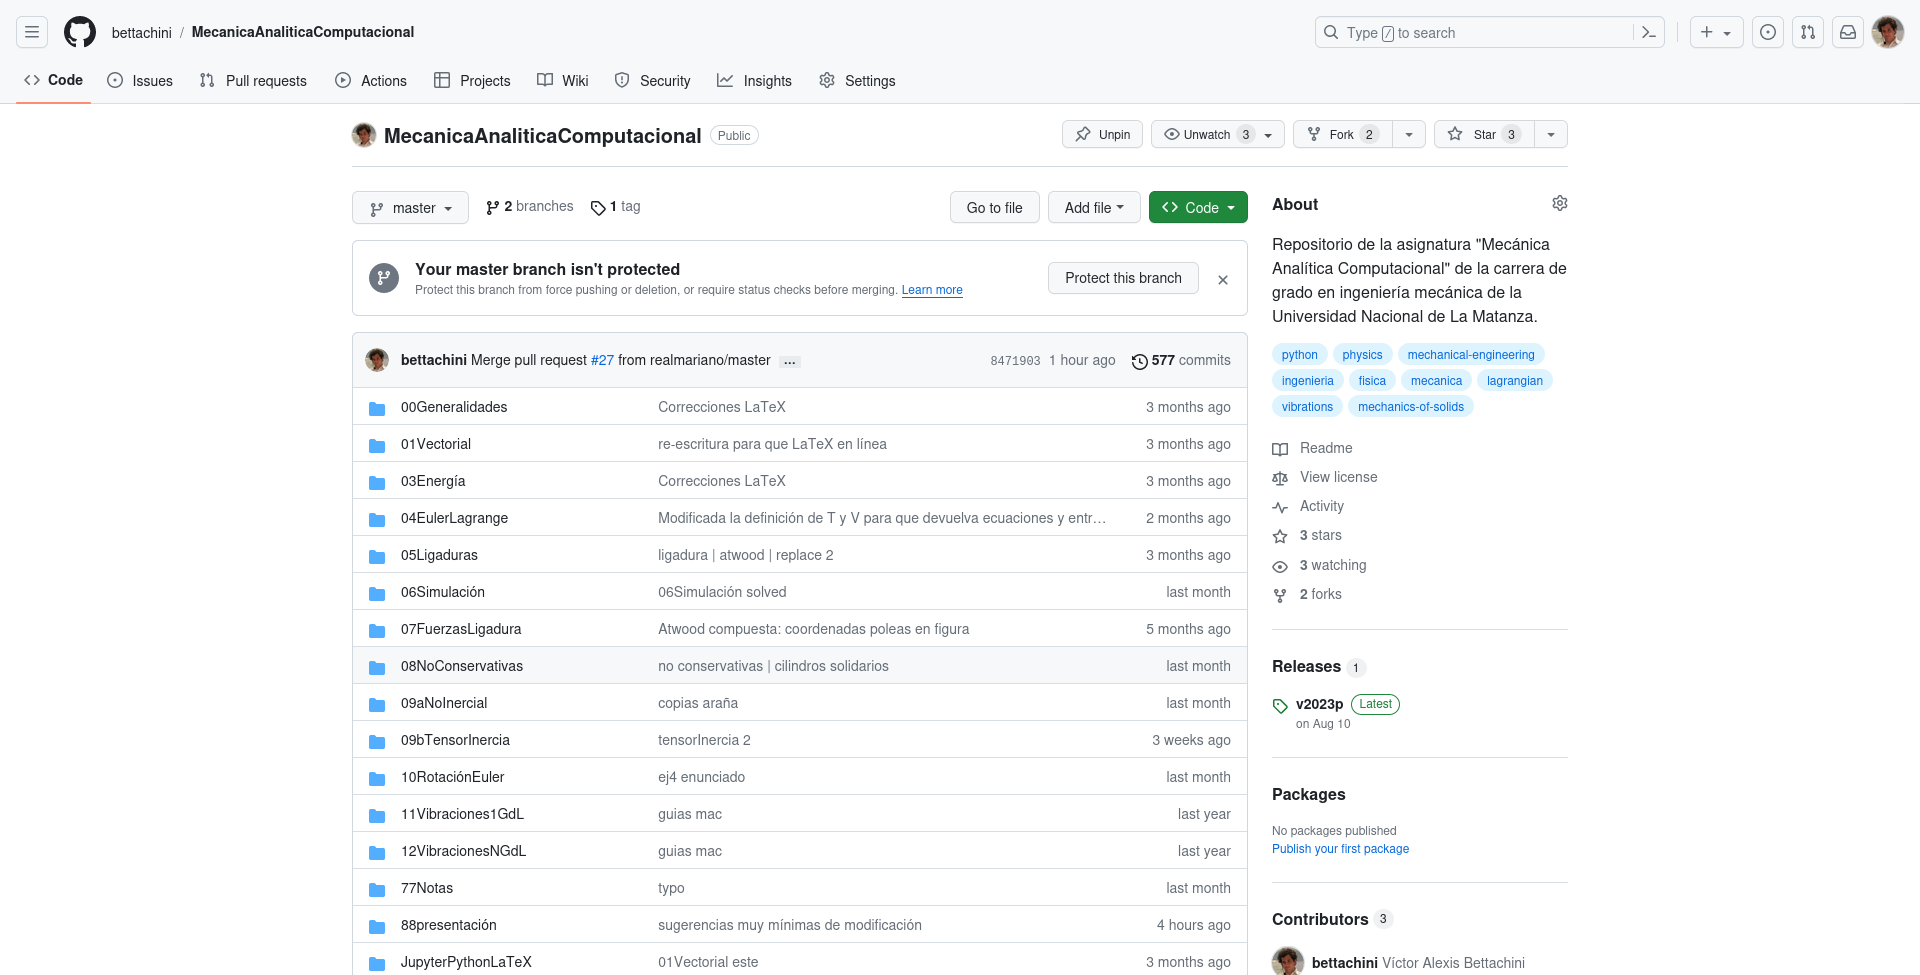
\includegraphics[width=3.5in]{figuras/repositorioGithub.png}
\caption{The students find the material organized in separate directories per class.}
\label{fig:github}
\end{figure}



% \subsection{Sistema de gestión de aprendizaje}

% En la UNLaM se utiliza la plataforma de comunicaciones de negocios Microsoft Teams para suplir la interacción en el aula con los alumnos con videoconferencias. Luego de terminada cada clase el video de las mismas se guarda en el almacenamiento en línea Microsoft OneDrive. Enlaces a estos y a los materiales de la clase alojados en el repositorio Git se  compartimentan en lo que el sistema llama canales respetando la misma numeración y denominación que en el repositorio Git. La figura \ref{fig:teams} muestra los contenidos que encabezan los desplegados para la décima clase.

% En cada canal se incluyen enlaces a:
% \begin{itemize}
%     \item guía de ejercicios prácticos
%     \item algún eventual apunte en PDF
%     \item ambas vías para ver los cuadernos Jupyter, la interactiva en Colab o estática en nbviewer
%     \item invitación a la videoconferencia o a su video una vez esta terminó
% \end{itemize}

% Microsoft Teams provee también los rudimentos de un sistema de gestión de aprendizaje (LMS por sus siglas en inglés) al permitir asignar tareas a alumnos con fechas límites de aceptación por parte del sistema. Los alumnos pueden cargar al sistema un enlace a su cuaderno en Colab o el mismo en formato .ipynb en el caso de que no se permita modificación del mismo con posterioridad a una fecha por cuestiones de evaluación.

% \begin{figure}[!ht]
% \centering
% 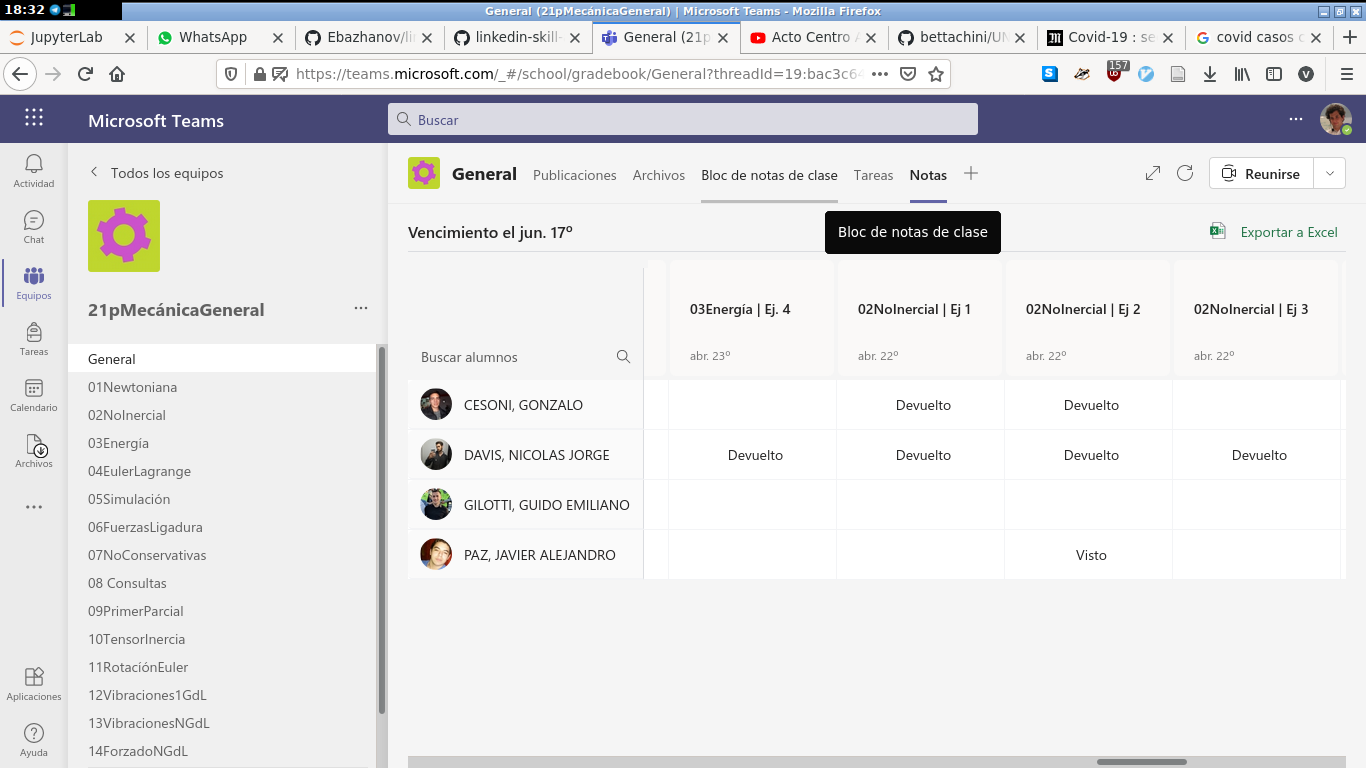
\includegraphics[width=3.5in]{figuras/notasTeams.png}
% \caption{Sendos canales por clase presentan los enlaces a su material.}
% \label{fig:teams}
% \end{figure}


\subsection{Learning Management System}
At UNLaM, the Microsoft Teams business communications platform is used to replace classroom interaction with students with videoconferencing. After each class, the videos are saved to Microsoft OneDrive online storage. Links to these and to the class materials hosted in the Git repository are compartmentalized into what the system calls channels, respecting the same numbering and naming as in the Git repository. Figure \ref{fig:teams} shows the contents that head the ones displayed for the tenth class.

Each channel includes links to:
\begin{itemize}
    \item practical exercise guide
    \item any occasional notes in PDF
    \item both ways to view Jupyter notebooks, interactive in Colab or static in nbviewer
    \item invitation to the videoconference or its video once it is over
\end{itemize}

Microsoft Teams also provides the rudiments of a Learning Management System (LMS) by allowing tasks to be assigned to students with acceptance deadlines by the system. Students can upload a link to their Colab notebook or the same in .ipynb format if modification is not allowed after a certain date for evaluation purposes.

\begin{figure}[!ht]
\centering
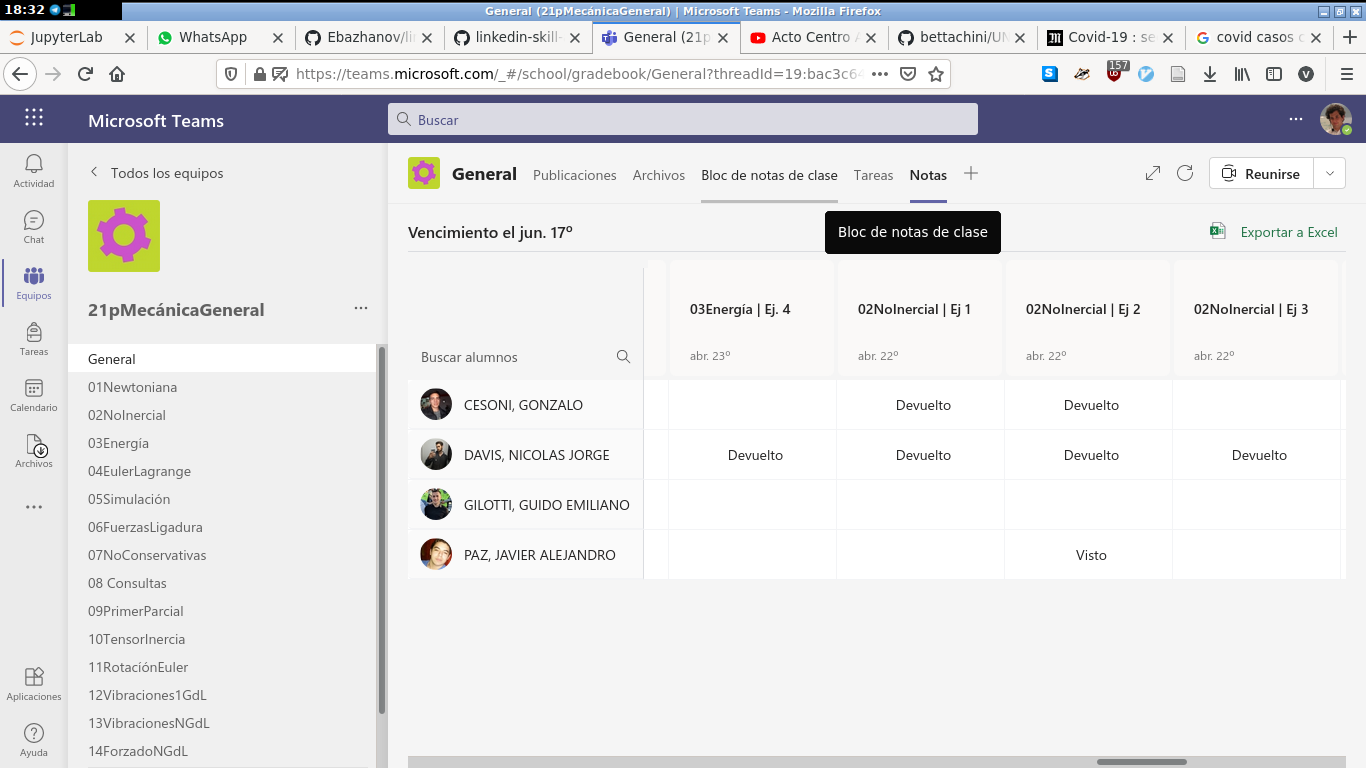
\includegraphics[width=3.5in]{figuras/notasTeams.png}
\caption{Separate channels per class present links to their material.}
\label{fig:teams}
\end{figure}
